\documentclass[reprint,amsmath,amssymb,aps,showpacs,superscriptaddress,prl]{revtex4-1}

\usepackage{graphicx}
\usepackage{bm}
\usepackage{epsfig}
\usepackage{amssymb}
\usepackage{amsfonts}
\usepackage{braket}
\usepackage{color}
\usepackage{epstopdf}
\epstopdfsetup{update}
\usepackage{hyperref}
\usepackage{float}
\restylefloat{table}
\usepackage{bibentry}
\usepackage{multirow}
\usepackage[caption=false]{subfig}
\newcommand{\ba}{\begin{eqnarray}}
\newcommand{\ea}{\end{eqnarray}}
\newcommand{\bd}{\begin{displaymath}}
\renewcommand{\v}[1]{{\bf #1}}
\newcommand{\nn}{\nonumber \\}

\graphicspath{{figures/}}% Put all figures in this directory.

\begin{document}
%
\title{Skyrmion}

%\pacs{75.78.-n, 75.10.Hk, 75.70.Kw, 75.78.Cd}
\maketitle

In the pure Rashba limit, we find the largest domain of stability for the hexagonal skyrmion crystal. In addition we also find a small sliver of stability for a square skyrmion lattice, together with an elliptic cone phase, distinct from the well-known vertical cone phase in the Dresselhaus limit. 

The Hamiltonian used takes the given form,

\ba && H_{\rm HDMZ} = -J \sum_{i\in L^2} \v n_i \cdot (\v n_{i+\hat{x}} + \v n_{i+\hat{y}} ) \nn
 & & + D \sum_i ( \hat{y} \cdot \v n_i \! \times \! \v n_{i\! +\! \hat{x}} - \hat{x} \cdot \v n_i \times \v n_{i\! +\! \hat{y}} )  - \v B \cdot \sum_i \v n_i .  \label{eq:HDMZ} \ea
%

With D=\sqrt6, and Anisotropy.
 
\begin{figure}[h]
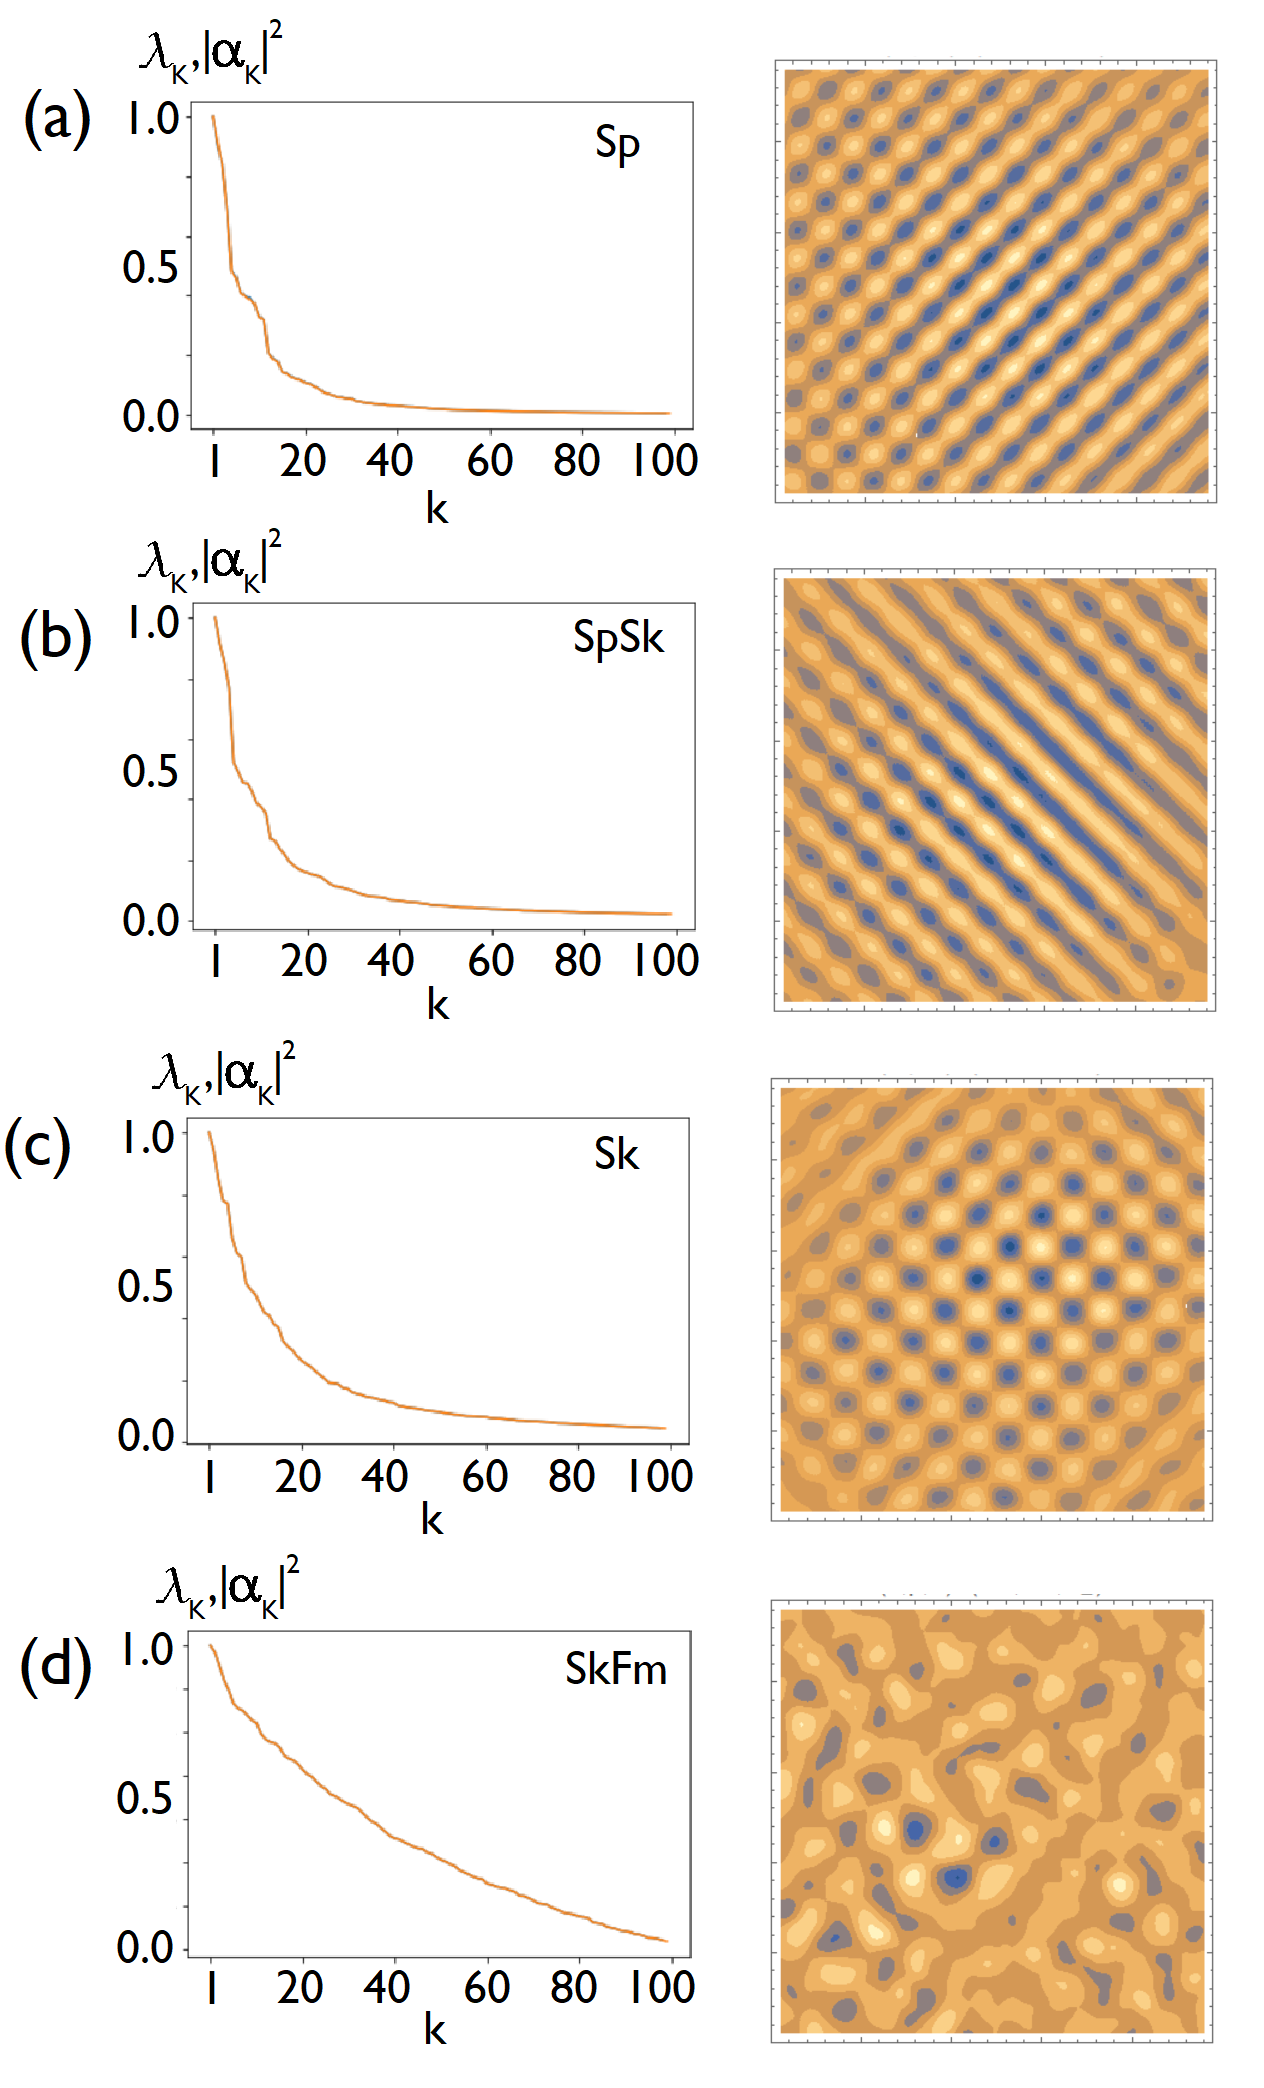
\includegraphics[scale=0.3]{fig1.png}
\caption{(left column) One hundred leading eigenvalues $\lambda_k$ of the correlation matrix, normalized by the largest value $\lambda_1$. Completely overlapping plots are obtained for average squares $\langle |\alpha_k |^2 \rangle / \langle |\alpha_1 |^2 \rangle$ [see Eq. (\ref{eq:alpha_k}) for definition]. (right column) The first ($k=1$) eigen-image of each phase. The $z$-component, $[{\bf I}_k ]_{iz}$, is used for the plot. Rest of the leading eigen-images are shown in SM. }\label{fig:0}
\end{figure}


\begin{thebibliography}{99}

\bibitem{} Skyrmions in Chiral Magnets with Rashba and Dresselhaus Spin-Orbit Coupling. James Rowland, Sumilan Banerjee, and Mohit Randeria1, https://arxiv.org/abs/1509.07508 (2015).


\end{thebibliography}

%\bibliographystyle{apsrev}
%\bibliography{reference}


\end{document}
